NaturalPad est une société innovante dont le domaine d'activité est encore à ses débuts. Si les jeux vidéo sérieux commencent à être connus du grand public et leur impact reconnu, ceux pour la santé ne sont pas encore assez nombreux ni assez largement acceptés. Mon travail de stage s'inscrit en réponse à cette constatation : il s'agit de proposer une méthode de conception de jeux vidéo pour la santé qui permettrait une simplification ou une amélioration de la conception de tels jeux. Proposer plus de jeux  thérapeutiques et/ou des jeux avec un impact santé de plus grande qualité contribuerait à améliorer leur diffusion et leur reconnaissance. Pour ces raisons, il était ainsi primordial de parfaire ma connaissance des différents domaines concernés.

Cette partie présente le résultat de mes recherches, des techniques et outils existants et comporte des notions importantes à connaître pour la conception de serious games pour la santé.

\subsection*{Méthode de travail}
Étendue sur plusieurs semaines, la réalisation de l'état de l'art était pour moi quelque chose de nouveau qui a nécessité une certaine organisation. Deux moments ont été importants : la phase de démarrage et l'arrêt des recherches. Commencer ces recherches alors que les sujets que je devais ou voulais couvrir étaient vastes et non clairement définis fut à la fois plaisant et compliqué. Bien que beaucoup de choses me semblaient intéressantes, la question était de savoir par où commencer. De la même manière, au fil de mes lectures, je découvrais de nouveaux liens et références présentant de nouveaux aspects qui eux-même renvoyaient vers d'autres solutions et articles. La difficulté était donc de juger quand mes connaissances sur un thème donné étaient suffisantes pour éviter de poursuivre d'interminables recherches, aussi intéressantes puissent elles être, le temps étant limité dans le cadre d'un stage de Master.
	\paragraph{}Au niveau des lectures abordées, ma source principale fut des articles scientifiques, suivie par des articles de magazines spécialisés et articles web notamment. Pour les thèmes médicaux, un certain nombre d'articles m'a été directement conseillé par des professionnels de la santé, articles à partir desquels j'ai ensuite pu compléter mon état de l'art en suivant les références. Par ailleurs, il est fréquent que certains auteurs ressortent régulièrement lorsqu'on effectue des recherches sur un thème donné, ce qui permet, en plus du nombre de citations des articles, de rapidement cerner quels sont les articles et chercheurs de référence dans le domaine.
	\paragraph{}Bien entendu, afin de rendre mes lectures efficaces, je me constituais pour chacune d'elle une fiche de lecture où noter les points importants : 
\begin{itemize}
	\item Titre ou source
	\item Auteur(s)
	\item Mots clefs
	\item Synthèse
	\item Jugement personnel ou remarques
	\item Références importantes
\end{itemize}

%% PART 1 : JEUX VIDEO
\subsection{Jeux Vidéo}
Durant mon stage, j'ai ainsi voulu comprendre pourquoi et comment un jeu vidéo est bon, quels en sont les mécanismes ou bien encore quels facteurs vont retenir le joueur. 
	%%Définition d'un Jeu 
	\subsubsection{Définition d'un Jeu}
Le jeu vidéo est un média participatif en pleine extension et de plus en plus largement accepté et plébiscité par la population. \\Dans sa définition, un jeu vidéo est une extension du jeu au monde numérique en utilisant les technologies informatiques. Il s'agit donc en amont de bien comprendre ce qu'est un jeu. \\Dans son travail d’analyse, Juul\cite{Juul05} donne une synthèse qui regroupe les points partagés par toutes les définitions existantes~:
\begin{quotation}
A game is a rule-based formal system with a variable and quantifiable outcome, where different outcomes are assigned different values, the player exerts effort in order to influence the outcome, the player feels attached to the outcome, and the consequences of the activity are optional and negotiable. 
\end{quotation}
\paragraph{Points clefs \\}
Les 6 points clefs identifiés par Juul sont :
\begin{itemize}
	\item les règles
	\item le résultat quantifiable variable
	\item la valorisation du résultat
	\item l’effort du joueur
	\item l’attachement du joueur au résultat (identifié par Gendler comme Alief, 2009)
	\item des conséquences négociables.
\end{itemize}

	\subsubsection*{Population de joueurs}
Le jeu vidéo est un média récent qui trouve ses origines dans le début de la seconde moitié du XX$^{eme}$ siècle. D'abord majoritairement accessibles sur des bornes d'arcade, les jeux vidéo se sont progressivement répandus avec la commercialisation de consoles de salon. Selon une étude commandée par le Centre National du Cinéma et de l'image animée\href{http://www.cnc.fr}{(CNC)}, c'est près de 60\% de la population française qui jouaient à des jeux vidéo au cours de l'année 2011\cite{Cnc11}. L'âge moyen des joueurs était alors de 34,7 ans et cette population constituée de 54,1\% d'hommes fin 2011\cite{Cnc11}. L'arrivée de la console Wii et de jeux orientés plus casuals\footnote{Se dit d'une personne ne jouant à des jeux vidéo que de manière occasionnelle. Peut aussi se dire d'un jeu dont la cible sont des joueurs occasionnels.} a permi en France une meilleure diffusion du média au sein de la population, qui accepte de plus en plus de se livrer à cette activité. Contrairement à ce que l'on pourrait croire, notamment à cause de leur méconnaissance des nouvelles technologies et du jeu vidéo plus spécifiquement, les seniors se prêtent aussi volontier à la pratique de ce loisir numérique. C'est une constation que nous avons pu vérifier par nous-même lors de nos différentes sessions de tests au centre hospitalier de Lapeyronie et dans une maison de retraite à Lille, mais aussi dans différentes lectures qui seront détaillées ci-après.
	
	%% Jeux vidéo et schéma comportementaux
	\subsubsection{Jeux vidéo et schémas comportementaux}
Pour expliquer l'attrait croissant de la population envers les jeux vidéo, il peut être intéressant de se tourner du coté des théories comportementales. Carl Rocray \cite{Rocr09} explique qu'en dépit de ses origines technologiques récentes, le jeu vidéo entretient d’anciens schémas de comportements, et cette influence est subtile. C’est le propre du jeu de nous divertir, non seulement de nos tracas réels, mais aussi de son influence sur nous pendant que nous jouons. Cette influence est évidente à travers le lien entre plaisir et apprentissage : l’effort diminue si on a du plaisir à le faire, et on peut même en oublier que nous apprenons.

\paragraph{}On se rend compte que la plupart des jeux vidéo peuvent être classés selon leur gameplay en ce que l'on appelle des types de jeux. Parmi les grands types connus, on retrouve par exemple les jeux d'action, les jeux de stratégie ou encore les jeux de simulation sportive. On trouvera en \href{types_jeux}{annexe} une liste plus complète de ces types de jeux vidéo classés en fonction de leur gameplay. \\

Il est intéressant de constater le lien entre les différents schémas comportementaux basiques et les types de jeux mettant en place des mécaniques stimulant nos instincts primaires [Rocray, 09]\cite{Rocr09}.

\paragraph{}
		\paragraph{Survie \\ \quad}
«Éliminer ou être éliminé». C’est la base de la majorité des jeux vidéo et probablement aussi le comportement le plus simple. Même les jeux de sports ou de cartes entretiennent cet instinct primaire, bien qu’il soit surtout manifeste dans les jeux de tir (\emph{Doom}, \emph{Gears of War}), les jeux de combats (\emph{Tekken}, \emph{Street Fighter}) et les «platformers» (\emph{Mario Bros}, \emph{Assassin’s Creed}).
		\paragraph{Gestion \\ \quad}
Il s’agit surtout de gestion de ressources, mais aussi d’équipement quand celui-ci est limité. Une bonne gestion permet habituellement de mieux survivre (meilleures ressources, équipement adéquat), ce qui nécessite une planification et une organisation stratégiques. On retrouve ce comportement dans les jeux de simulation (\emph{SimCity}, \emph{Civilization}), de «Real Time Strategy» (\emph{Warcraft}, \emph{Starcraft}) et ceux qui visent un certain réalisme (\emph{Arma}, équipement limité dans \emph{Resident Evil}).
		\paragraph{Responsabilisation d’autrui \\ \quad}
Ce comportement fait appel à une sorte d’instinct parental où nous devons assurer la survie d’un autre joueur ou le bien-être d’un avatar virtuel qui nous ramène en fait à nous-même. Il est d’abord présent dans les jeux de simulation (\emph{The Sims}, \emph{Tamagotchi}) et ceux de coopération (\emph{Army of Two}, \emph{Left 4 Dead}).
		\paragraph{Résolution de puzzles \\ \quad}
Mystères à résoudre (\emph{Myst}), problèmes de logique faisant appel à nos capacités cognitives (\emph{Brain Challenge}), voire comment empiler des formes (\emph{Tetris}) ou aligner des couleurs (\emph{Bejeweled}), il s’agit toujours de trouver la solution la plus efficace à un problème donné.
		\paragraph{Réflexes et dextérité \\ \quad}
La plupart des jeux font appel à cet instinct également lié à la survie.
Surtout lié à la coordination «oeil-main» et à la précision d’actions souvent rapides (voir entre autres les «Quick-Time Events»), il est aussi lié à la maîtrise d’un outil, c’est-à-dire la manette de jeu. On le retrouve dans les jeux de rythme (\emph{Guitar Hero}, \emph{Rock Band}), mais aussi dans les jeux de Survie cités plus haut et tous les jeux de sports.
		\paragraph{Système de récompenses \\ \quad}
La grande majorité des jeux vidéo utilise ce système de la carotte au bout du bâton pour diriger les actions du joueur. Il est donc étroitement lié à la motivation et à la gratification de comportements donnés. Voir entre autres \emph{Little Big Planet} et \emph{Diablo}, ainsi que la mode assez récente des Trophées, Succès et autres «Achievements».
		\paragraph{Système d’améliorations \\ \quad}
Une autre mécanique liée à la Survie et à la courbe de difficulté des jeux. En bref, il s’agit de devenir plus fort pour défaire des adversaires toujours plus forts. C’est la base des «Role-Playing Games» (\emph{World of Warcraft}, \emph{The Elder Scrolls}) et de certains jeux de «Shooter» (pour améliorer ses armes).

		\paragraph{}
Il est probable que d’autres comportements soient ainsi entretenus par le médium vidéo-ludique. Les sept types de mécaniques décrites ci-haut montrent néanmoins comment les jeux vidéo nous font répéter d’anciens schémas de comportement.

	%%State of Flow
	\subsubsection{L'état de flux ou expérience optimale}
Le state of flow ou état de flux, fut originellement décrit par Csikszentmihalyi\cite{Csik88} dans les années 80 bien qu'il utilisa déjà ce terme dans ses recherches précédentes\cite{Csik75}. C'est l'état dans lequel une personne peut se trouver, proche de l’extase (dans le sens “se trouver à coté de”) complètement immergée dans ce qu'elle fait, dans un état maximal de concentration. Cette personne éprouve alors un sentiment d'engagement total et de réussite. Dans cet état, on est alors hyper compétent, naturellement, inconsciemment dans ce qu’on est en train de faire : musique, sport, travail, jeux, lecture, etc. Cet état est commun chez les personnes exerçant une activité répétitive et/ou demandant de gros efforts physiques ou psychiques. On est comme détaché de son corps, que l’on voit agir tout seul. On est alors capable d’accomplir des choses qu’on serait incapable de réaliser consciemment de manière contrôlée. S’il n’est pas interrompu, cet état d'expérience optimale peut durer une dizaine ou une vingtaine de minutes.

\paragraph{}
L’état de flux est l’une des raisons pour lesquelles on joue aux vidéo [Murphy, 2011]\cite{Murp11}. Leur but est de divertir en jouant sur la motivation du joueur, ce qui est lié au flow state. Le jeu, au moyen d’une balance entre compétences et challenge, maintient la vivacité d’esprit du joueur, avec une motivation importante et une attention forte[Rutledge, 2012]\cite{Rutl12}. Être dans cet état de flux permet donc au joueur une meilleure expérience de jeu augmentant son ressenti et son souhait de continuer à jouer[Chen, 07]\cite{Chen07}. Pour rentrer dans cet état de grâce, les deux états d’esprit les plus proches sont l’excitation et le contrôle, le flow state se trouvant à l’intersection de ces deux noeuds. On peut donc essayer de mettre le joueur dans ces états là si on cherche à stimuler ce flow state.

\begin{figure}[h!]
	\centering
	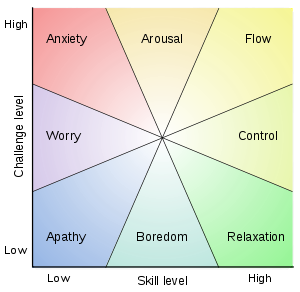
\includegraphics[width=9cm]{images/state_of_flow.png}
	\caption{Positionnement entre les humeurs et l'état de flux [Csikszentmihalyi, 1997]\cite{Csik97}}
	\label{state_of_flow}
\end{figure}

\paragraph{}
Csikszentmihalyi identifie les caractéristiques de l’état de flux~:
\begin{enumerate}
   \item prédispositions ou caractéristiques propices pour atteindre cet état~:
         \begin{itemize}
            \item des objectifs clairs et précis
            \item équilibre entre difficulté de la tâche et compétences de l’acteur (joueur)
            \item l’activité est en soi une source de satisfaction (amusante ou pour laquelle le joueur est impliquée)
         \end{itemize}
   \item conséquences et caractéristiques~:
   	\begin{itemize}
            \item hyperfocus, concentration exacerbée sur une action précise
            \item perte de la conscience de soi
            \item perception du temps modifiée
            \item rétroaction immédiate : prise de conscience de l’action effectuée, pour ajuster les suivantes
            \item sentiment de contrôle de la situation
	\end{itemize}
\end{enumerate}